\documentclass[]{report}
\usepackage{listings}
\usepackage[ngerman]{babel}
\usepackage[utf8]{inputenc}
\usepackage[pdftex]{graphicx}     
\usepackage{booktabs}
\usepackage{color}
\usepackage{tabulary}
 \lstset{language=Java,
          showstringspaces=false,
          frame=single,
          numbers=left,
          basicstyle=\ttfamily,
          numberstyle=\tiny
        }
% Title Page
\title{MISS \\ Mac-based Identification and Signaling Service}
\author{Fabian Schwab (fabian.schwab@uni-ulm.de)}
\begin{document}
\maketitle

%\begin{abstract}
%\end{abstract}
\chapter{Einleitung}
Der \textit{mac-based identification and signaling service} ist ein für Android geschriebener Hintergrunddienst, welcher es ermöglicht mobile oder stationäre WLAN Geräte zu erkennen. Der Service unterscheidet zwischen mobilen Geräten, die hier als \textit{Clients} bezeichnet werden und Stationen den sogenannten \textit{Stations}. Hierbei sind die \textit{Clients} Geräte die sich mit einem WLANs verbinden und \textit{Stations} Geräte, die solch ein Netzwerk aufspannen. Je nach Typ werden verschiedene Informationen gesammelt und zurückgegeben, welche in Kapitel \ref{airodump-ng} genauer erläutert werden.\\
Sobald sich eines der gesuchten Geräte in der Nähe befindet und erkannt wird, wird eine Benachrichtigung über dessen Fund ausgelöst.
\chapter{Grundlagen}
Um die Funktionsweise des Service genauer verstehen zu können, sollten zunächst einige Grundlagen erklärt werden. In diesem Abschnitt werden die vom Service genutzten Technologien kurz beschrieben. Da dies keine vollständige Beschreibung darstellt, sollten die Technologien in ihren Grundzügen bekannt sein. 
\section{Kabellose Kommunikation}
Die Anzahl der Geräte die mithilfe von WLAN kommunizieren nehmen ständig zu. Bei einem Großteil dieser Geräte wird das \textit{WNIC}\footnote{Wireless Network Interface Controller}, manchmal trotz limitierter Ressourcen, nicht abgeschaltet. Trotz verschlüsselter Verbindungen werden definiert durch den \textit{IEEE 802.11} Standard einige Daten in Klartext übertragen. Diese Daten werden von MISS genutzt um Geräte in der Nähe zu erkennen und bekannte zu identifizieren. \\
Durch den \textit{IEEE 802.11} Standard werden auf der Sicherungsschicht des \textit{OSI-Modell} Datagramme, sogenannte \textit{Frames} definiert welche in spezielle Teile unterteilt sind. Jeder \textit{Frame} enthält ein \textit{MAC header} Feld, in dem die Absender MAC-Adresse im Klartext dargestellt ist. Durch belauschen der umliegenden Kommunikation kann so nach einer bestimmten MAC-Adresse gesucht werden. \\
Aber nicht nur Geräte die im Moment Daten austauschen können erkannt werden, sonder auch Geräte die inaktiv sind. Jedes WLAN fähige Gerät senden abhängig von der Implementierung des \textit{WNIC} Treibers periodische Pakete aus. Diese Pakete gehören zu der Gruppe der \textit{Managementframes}. \\
Bei den \textit{probe request frames} handelt es sich um Pakete die von \textit{Clients} gesendet werden um Informationen über Netzwerke zu sammeln. Durch die Angabe einer \textit{SSID}\footnote{Service Set Identifier} kann im Kommunikationsbereich des Gerätes nach bestimmten Netzwerken gesucht werden oder durch Angabe der \textit{boradcast SSID} kann nach allen Netzwerken gesucht werden die dieses Paket empfangen und darauf Antworten. Diese Pakete werden periodisch versendet egal ob das Gerät bereits mit einem Netzwerk verbunden ist oder nicht.\\
\textit{Stations} senden sogenannte \textit{beacon frames} aus. Damit geben sie periodisch ihre Präsenz, \textit{SSID} und andere Parameter bekannt. \\
Im Standard Betriebsmodus eines \textit{WNIC} ist es nicht vorgesehen, dass Pakete, die an andere MAC-Adressen gerichtet sind an höhere Schichten weitergeleitet werden. Diese Pakete werden bereits auf der zweiten Schicht dem \textit{Data Link Layer} verworfen. Damit aber auch diese Pakete weitergeleitet werden, ist es notwendig den Betriebsmodus des \textit{WNIC} auf den sogenannten \textit{Monitor Mode} zu setzten. Dieser Mode wird über den Treiber des \textit{WNIC} eingestellt um muss dort auch implementiert sein. 
\subsection{Airodump-ng}\label{lab:airodump-ng}
\textit{Airodump-ng}\footnote{http://www.aircrack-ng.org/doku.php?id=airodump-ng} ist ein Kommandozeilenprogramm welches für das erfassen von \textit{IEEE 802.11 frames} genutzt wird und ein Teil der \textit{Aircrack-ng suit}\footnote{http://www.aircrack-ng.org} ist. Mit diesem Programm lassen sich Log-Dateien erstellen welche Informationen über alle erfassten \textit{Stations} und \textit{Clients} enthalten. Eine Auszug von solch einer Log-Datei ist in Abbildung \ref{fig:log_file} zusehen. Die nachfolgenden Auflistungen beschreiben stichpunktartig die erfassbaren Daten für \textit{Stations} und \textit{Clients}.\\ \\
\begin{figure}
    \centering
    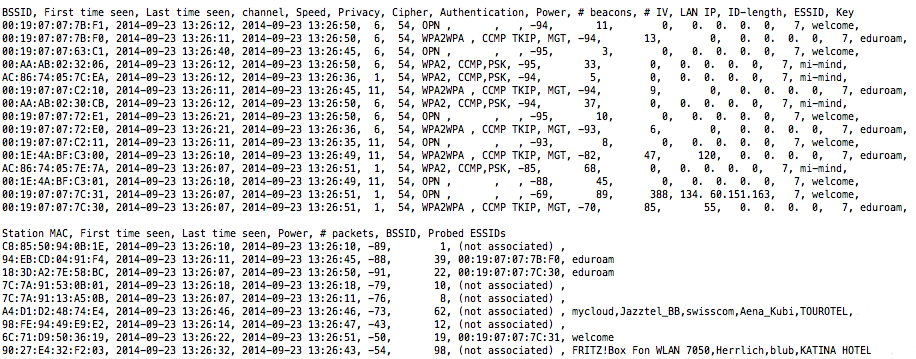
\includegraphics[width=5.0in]{bilder/log.png}
    \caption{Mit airodump-ng erstellte Log-Datei}
    \label{fig:log_file}
\end{figure}
\begin{center}
  \begin{tabulary}{\textwidth}{l | L}
\toprule
Erfassbare \textit{Station} Daten & Beschreibung \\
\midrule
BSSID & MAC-Adresse der \textit{Station} \\
First time seen & Datum und Uhrzeit der ersten Kontakts \\
Last time seen & Datum und Uhrzeit des letzten Kontakts \\
channel &  Kanal auf der die \textit{Station} sendet \\
Speed & Übertragungsgeschwindigkeit in MBit/s\\
Privacy & Privatsphäreneinstellungen \\
Cipher & Art der Verschlüsselung \\
Authentication & Genutztes Authentifizierungsprotokoll \\
Power & Signalstärke \\ 
\# beacons & Anzahl der Empfangenen \textit{beacon frames}\\
\# IV & Anzahl der Erkannten Initialisierungsvektoren \\
LAN IP &  IP Adresse \\
ID-length & Länge der ESSID \\
ESSID & Netzwerkname \\
Key & Netzwerkschlüssel falls bekannt (genutzt mit aircrack-ng) \\
\bottomrule
\end{tabulary}
\end{center} 
\begin{center}
  \begin{tabulary}{\textwidth}{l | L}
\toprule
Erfassbare \textit{Client} Daten & Beschreibung \\
\midrule
Station MAC & MAC-Adresse \textit{Clients} \\
First time seen & Datum und Uhrzeit der ersten Kontakts \\
Last time seen & Datum und Uhrzeit der letzten Kontakts \\
Power & Signalstärke \\
\# packets & Anzahl der Empfangenen \textit{frames} \\
BSSID & BSSID mit dem der \textit{Client} verbunden ist \\
Probed ESSIDs & ESSID die der \textit{Client} sucht \\
\bottomrule
\end{tabulary}
\end{center}
\section{Android}
Bevor der eigentliche Hintergrunddienst installiert werden kann und funktionsfähig ist, müssen einige Vorbereitungen getroffen werden. Da Google in seinem offenen Betriebssystem Android keine Möglichkeit bietet einen \textit{Monitor Mode} zu aktivieren, implementieren die meisten Hersteller diesen auch nicht für ihre WLAN Module.\\
Aktuell gibt es kein Android Gerät welches einen \textit{WNIC} besitzt, für den es einem vom Hersteller implementierten \textit{Monitor Mode} gibt. Für bestimmte Chipsätze des Herstellers Broadcom gibt es eine kleine Gruppe von Programmierer, die für die Chipsätze \textit{BCM4330} und \textit{BCM4329} eine neue Firmware geschrieben haben um eben diesen Modus zu aktivieren. Momentan werden folgende Geräte mit diesem Chipsatz unterstützt:
\begin{itemize}
\item Samsung Galaxy GS1 mit Cyanogen 7
\item Samsung Galaxy GS2 mit Cyanogen 9 oder Cynaogen 10
\item HTC Nexus One mit Cyanogen 7
\item Asus Nexus 7 mit Cyanogen 7
\end{itemize}
\subsection{Cyanogen}
Alle zuvor ausgelisteten Geräte nutzen Cyanogen\footnote{http://www.cyanogenmod.org}. Cyanogen ist eine erweiterte \textit{open source} Firmware Distribution für Smartphones und Tablets welche auf den Android Betriebssystem basiert. Diese bietet Eigenschaften und Erweiterungen die es in der offiziellen oder in der des Herstellers ausgelieferten Firmware nicht gibt. \\
Um Cyanogen auf einem Unterstützten Gerät zu installieren, muss es zuvor \textit{gerootet} werden. Diese bedeutet, das man alle Rechte erlangt was normalerweise auch aus Sicherheitsgründen so nicht vorgesehen ist. 
\subsection{bcmon.apk}
Nachdem das Gerät \textit{gerootet} wurde und Cyanogen installiert wurde. Wird das kleine Programm \textit{bcmon}\footnote{http://bcmon.blogspot.de} installiert. Mithilfe dieses Programms, welches die neue Firmware für den \textit{WNIC} enthält, kann der \textit{Monitor Mode} aktiviert werden. Anschließend ist das Gerät für die Verwendung des MISS Hintergrunddienstes vorbeireitet. 
\chapter{Architektur und Implementierung}
In diesem Kapitel wird zunächst die grundlegende Architektur des verwendeten Dienstes erläutert und anschließend auf die Implementierung eingegangen. Dieses und nachfolgende Kapitel setzten voraus, dass Grundlagen der Programmierung in Java und Android bekannt sind. Sind diese nicht bekan  nt, wird an dieser Stelle auf die Android-Entwicklerseite\footnote{http://developer.android.com} verwiesen. 
\section{Architektur}
\subsection{Android IntentService}
Ein Service ist eine im Hintergrund laufende Komponente welche keine direkte Interaktion mit einem Nutzer besitzt. Da ein Service kein Benutzeroberfläche benötigt, ist ein dieser auch nicht an den Lebenszyklus einer \textit{activity} gebunden. Im Allgemeinen werden Services genutzt um wiederkehrende und potentiell lange andauernde Aufgaben zu erledigen wie Beispielsweise das herunterladen von Inhalten aus dem Internet oder das aktualisieren von Daten. Ebenfalls werden Services mit einer höheren Priorität als sich im Hintergrund befindlichen Anwendungen ausgeführt und daher ist es unwahrscheinlicher, dass sie vom Betriebssystem abgeschaltet werden. \\
Zusätzlich können Services unter Android so Konfiguriert werden, dass sie neu gestartet werden sollte das Betriebssystem sie beenden. \\
Da der in diesem Projekt genutzte Service nicht immer aktiv sein soll, wird hier auf eine besondere Art eines Service zurückgegriffen. Bei dieser Art von Hintergrunddienst handelt es sich um einen in \textit{intentService} welcher von der Klasse \textit{Service} erbt. Der Lebenszyklus eines \textit{intentService} ist in Abbildung \ref{fig:lifetime} abgebildet. Hierbei wird ersichtlich, dass diese Art von Service nicht immer im Hintergrund aktiv ist. Nur wenn ein Client an der Service gebunden ist wird, ist dieser aktiv. Im Gegensatz zu seiner Basisklasse, wobei ein Aufruf von \textit{stopService()} genügt um diesen zu beenden, wird ein \textit{intentService} erst beendet, wenn sich alle Clients entbunden haben.
\begin{figure}
    \centering 
    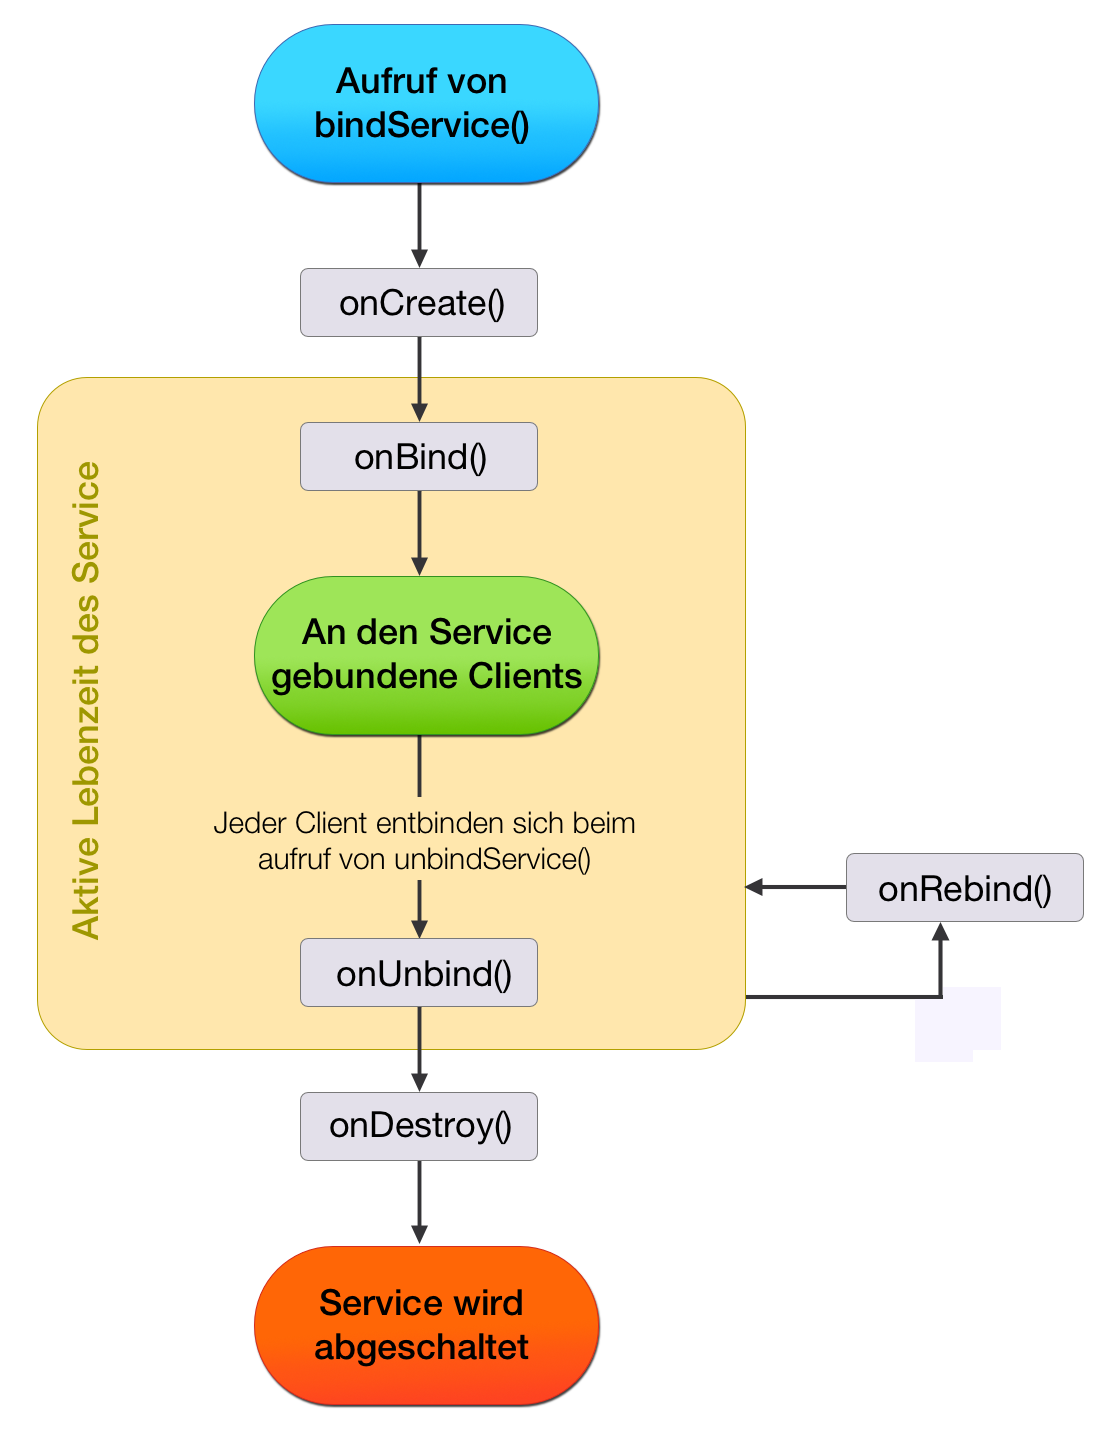
\includegraphics[width=3.0in]{bilder/intentservice.png}
    \caption{Lebenszyklus eines \textit{intentService}}
    \label{fig:lifetime}
\end{figure}
\subsection{Service Logik}
Der Aufbau des Service wie er Implementiert werden soll ist in Abbildung \ref{fig:uml} ersichtlich. Bindet sich eine Anwendung am Service wird dieser, falls er noch nicht aktiv ist, gestartet. Der Service verfügt über einen eigenen Thread, welcher die eigentliche Arbeit übernimmt. Dies ermöglicht ein sofortiges abarbeiten weiterer Anfragen von bereits gebundenen Anwendungen oder wenn sich weitere Anwendungen an den Service binden möchten. \\
Aus Effizienzgründen wird der Thread nur gestartet wenn Geräte gesucht werden. Diese werden zu suchenden Geräte werden an den Service übermittelt, der daraufhin den Thread nach bedarf startet oder stoppt. \\
Die Aufgabe des Threads ist es alle Geräte in der Nähe zu erfassen. Dabei sollen alle zu erfassenden Daten, wie in Abschnitt \ref{lab:airodump-ng} gezeigt, erfasst werden. Anschließend werden die gefunden Geräte mit den gesuchten Verglichen. Befindet sich ein gesuchtes unter den gefunden so benachrichtigt der Thread den Service. Der Service benachrichtigt die entsprechende Anwendung über den Fund des angefragten Gerätes. \\ 
Je nach Implementierung der Zielanwendung entscheidet diese über das weitere vorgehen. In der Regel wird davon ausgegangen das die Anwendung eine Aktion auslöst und das gesuchte Gerät nicht mehr benötigt wird und es dem Service mitteilt.  
Durch eine Nachricht an den Service wird das zuvor gescuhte Gerät entfernt.\\
Der Service überprüft bei jedem Empfang einer Nachricht ob der Arbeiter-Thread gestartet werden muss oder nicht. Das entscheiden Kriterium ist, ob sich gesuchte Geräte im Service befinden. Antwortet eine Anwendung auf den Fund eines seiner Gesuchten Geräte nicht, wird davon ausgegangen das die Anwendung unerwartet beendet wurde. Der Service entfernt die Anwendung und all ihrer Geräte welche im Zusammenhang mit ihr stehen.\\
Befinden sich keine gesuchten Geräte im Dienst, beendet dieser den Arbeiter-Thread. Haben sich alle Anwendungen ordnungsgemäß vom Service abgemeldet oder wurden durch eine ausbleibende Antwort entfernt, beendet sich der Service selbst da er nicht mehr benötigt wird.
\newpage
\begin{figure}[h!]
    \centering 
    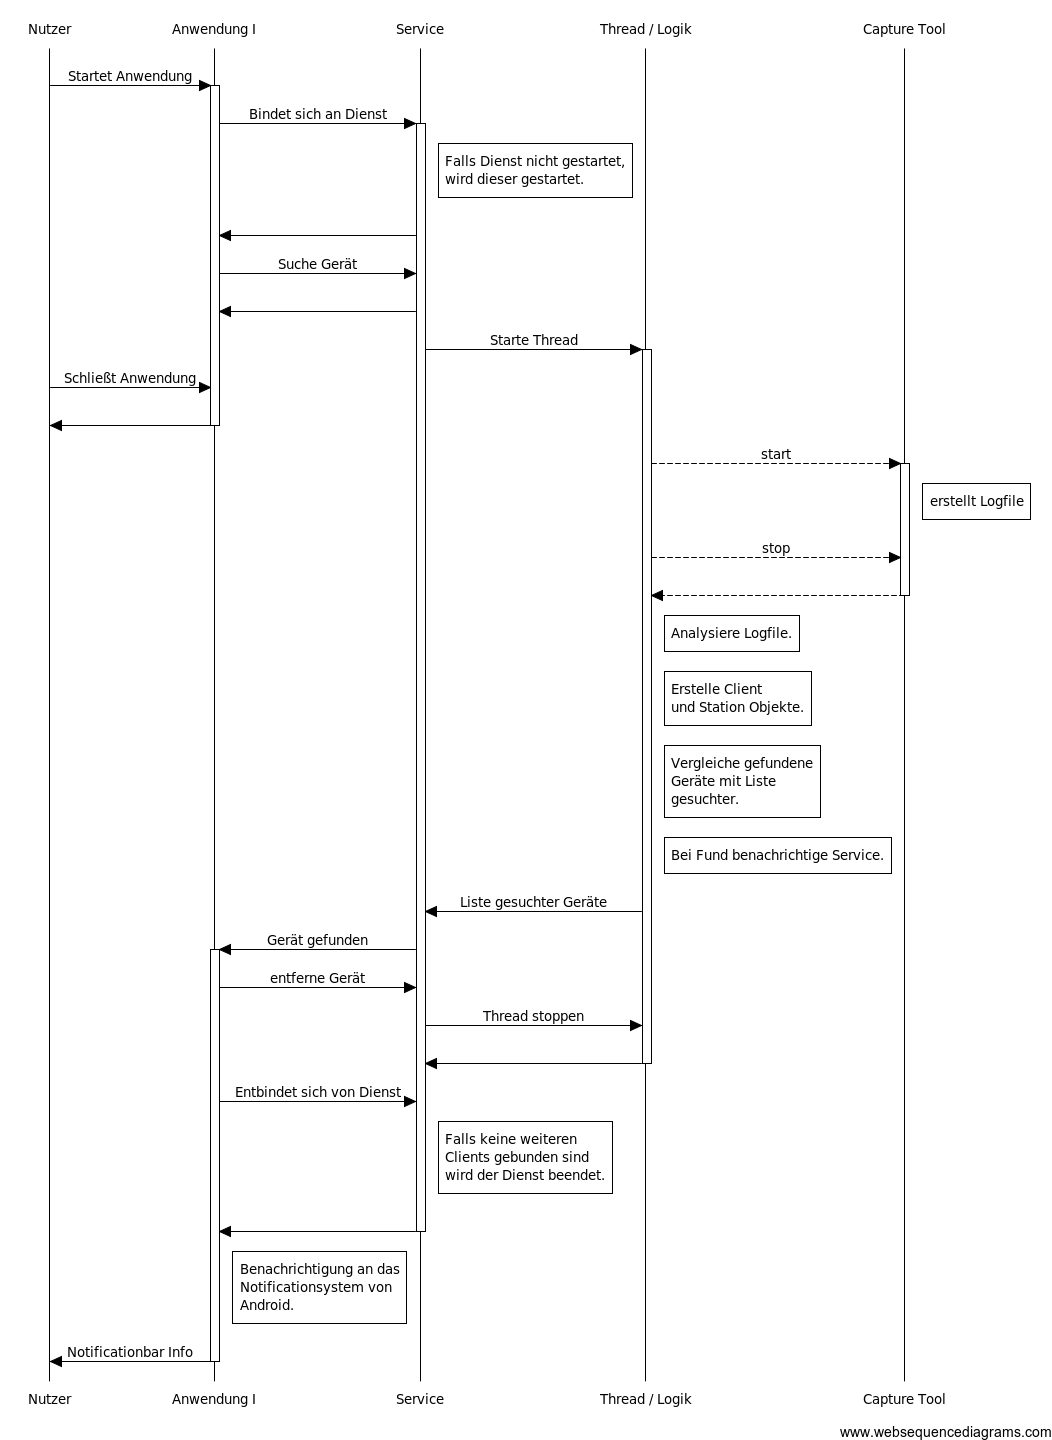
\includegraphics[width=5.0in]{bilder/uml.png}
    \caption{Anwendungsfall und Lebenszyklus des MISS als UML-Sequenzdiagramm.}
    \label{fig:uml}
\end{figure}
\section{Implementierung}
Für die Implementierung der voran gezeigten Architektur wurde das Eclipse ADT\footnote{http://developer.android.com/sdk/index.html} verwendet. Als Zielgerät wurde das Samsung Galaxy GS1 mit Cyanogen 7 gewählt. Hierbei war zu beachten, das bei der Programmierung nur Eigenschaften bis API Level 10 zu Nutzen sind. Dies liegt an der geringen Android Version 2.3.3 welche dem Cyanogen 7 Mod zu Grunde liegt. \\
Da im späteren Betrieb des Service Skripte benötigt werden, wurden diese zur besseren Kapselung und Entwicklung als \textit{.sh} Datei in \textit{assets} gespeichert. Dies hat den entscheidenden Vorteil, dass die Skripte nicht vom Nutzer separat nach der Installation im Programmverzeichnis abgelegt werden müssen sondern programmatisch generiert werden können.\\
Folgende Skripts werden bei der Installation erstellt:
\begin{itemize}
\item removeCaptureFiles.sh
\item startCapture.sh
\item stopCapture.sh
\end{itemize}
Alle Skripte werden ausschließlich von später gezeigten Arbeiter-Thread genutzt. Wobei \textit{removeCaptureFiles.sh} lediglich zum entfernen der anfallenden Log-Datei genutzt wird. \\ Das Starten und Stoppen von \textit{airodump-ng} wird durch die beiden anderen Skripte veranlasst, wobei \textit{startCapture.sh} wie in Listing \ref{lst:sh} einige Parameter enthält. Unter anderem wird hier das Ausgabeformat festgelegt und der \textit{WNIC} Name angegeben. Des weiteren werden die Umgebungsvariablen ergänzt um gewisse Bibliotheken für \textit{airodump-ng} bereitzuhalten um eine fehlerfreie Ausführung zu gewähren.
\begin{lstlisting}[caption={Airodump-ng Parameter}\label{lst:sh},captionpos=t] 
export PATH=
 $PATH:/data/data/com.bcmon.bcmon/files/tools
export LD_LIBRARY_PATH=
 $LD_LIBRARY_PATH:/data/data/com.bcmon.bcmon/files/libs
export LD_PRELOAD=
 /data/data/com.bcmon.bcmon/files/libs/
 libfake_driver.so
airodump-ng -w /datadata/de.uulm.miss/files/capture 
 --output-format csv -w capture wlan0 2>&1
 \end{lstlisting}
In der nachfolgenden Auflistung werden alle Klassen und eine dazugehörige Beschreibung des MISS aufgeführt.\\ \\
\begin{center}
  \begin{tabulary}{\textwidth}{l | L}
  \toprule
  Klassenname & Beschreibung \\
  \midrule
  MainActivity.java & Wird nur bei der Installation geöffnet und erzeugt alle nötigen Skripte.\\
  MISService.java & Nimmt Anwendungsanfrage entgegen und erzeugt und kontrolliert den Arbeiter-Thread. \\
  ScanLogic.java & Arbeiter-Thread der mithilfe der Skripte alle Geräte findet und mit zu suchenden Vergleicht. \\
  FileParser.java & Erstellt Client und Station Objekte anhand des Logfiles. \\
  Client.java & Objekt welche alle für Clients erfassbaren Daten enthält. \\
  Station.java & Objekt welche alle für Stations erfassbaren Daten enthält. \\ 
  ScanOrder.java & Enthält die Liste von gesuchten Stations und Clients. \\
  \bottomrule
  \end{tabulary}  
\end{center}
Auf eine ausführliche Beschreibung der Funktionen und Parameter wurde an dieser Stelle verzichtet, da diese aus dem Quellcode entnommen werden kann. Um diesen Service zu Nutzen kann die beiliegende Anwendung, \textit{PAR} welche in Abschnitt \ref{lab:par} erläutert wird, genutzt werden. \\
Die Basisfunktionen die der Service nach außen hin bietet werden im nächsten Kapitel \ref{lab:usage} erklärt. 
\subsection{Nutzung des Service}\label{lab:usage}
Für die Nutzung des Service müssen folgende Punkte erfüllt sein:
\begin{itemize}
\item Ein unterstützter Chipsatz (BCM4330 bzw. BCM4329) wurde verbaut.
\item Das Gerät ermöglicht \textit{root} zugriff
\item Eine kompatible Cyanogen Firmware ist aufgesetzt
\item Die bcmon Anwendung ist installiert.
\item MISS installiert und \textit{root} Rechte bewilligt.
\item Via bcmon aktivierter \textit{Monitor Mode}
\end{itemize}
\subsection{Anwendungsprogramm PAR}\label{lab:par}
\end{document}